%%%%%%%%%%%%%%%%%%%%%%%%%%
% A template for PhD Thesis
% Systems Security Group
% Coventry University
% 2020
%%%%%%%%%%%%%%%%%%%%%%%%%%


\documentclass[12pt,oneside]{book}
\usepackage[margin=1.2in]{geometry}
\usepackage[toc,page]{appendix}
\usepackage{graphicx}
\usepackage[square,numbers]{natbib}
\usepackage{lipsum}
\usepackage{caption}
\usepackage{pdfpages}
\usepackage{etoolbox}
\usepackage{setspace}
\AtBeginEnvironment{quote}{\singlespacing\small}
\begin{document}

\captionsetup[figure]{margin=1.5cm,font=small,labelfont={bf},name={Figure},labelsep=colon,textfont={it}}
\captionsetup[table]{margin=1.5cm,font=small,labelfont={bf},name={Table},labelsep=colon,textfont={it}}
\SetLipsumDefault{1}

\frontmatter

\begin{titlepage}


% -------------------------------------------------------------------
% You need to edit the details here
% -------------------------------------------------------------------

\begin{center}
{\LARGE University Of Crete}\\[0.25cm]
{\Large Department of Computer Science}\\[1.5cm]
\linespread{1.2}\huge {\bfseries Feature Extraction for Multi-layer Graph Link Prediction}\\[1.5cm]
\linespread{1}

\includegraphics[width=6.5cm]{Thesis/images/UoC_logo.png}\\[1.5cm]
{\Large\bf  Dimitrios Andreas Vogiatzidakis}\\[1cm]
{\large \emph{Supervisor:}   Polyvios Pratikakis}\\[0.25cm]% if applicable
\vspace{\fill}
\large A thesis submitted in partial fulfilment of the University's requirements\\ for the degree of Bachelor of Science\\[1cm]
\today
\end{center}

\end{titlepage}


% -------------------------------------------------------------------
% Declaration
% -------------------------------------------------------------------


% \includepdf[pages=-]{forms/form.pdf}

%\chapter*{\Large \center Acknowledgement}

\lipsum[5]

% -------------------------------------------------------------------
% Abstract
% -------------------------------------------------------------------

\chapter*{\Large \center Abstract}

Data sets can naturally be represented as graph where nodes represent instances and links represent relationships between those instances.A fundamental issue with these types of data is that links may incorrectly exist between unrelated nodes or that links may be missing between two related nodes. The goal of link prediction is to predict those irregularities between the nodes of the graph and also possible future links. \newline 
This thesis tries to reproduce the feature extraction algorithm of TwitterMancer[1] using the Apache Flink framework. Apache Flink is a framework and distributed processing engine for stateful computations over unbounded and bounded data streams, designed to run in all common cluster environments and perform computations at in-memory speed and at any scale. We will use this framework to speedup the process of feature extraction and as a result, analyze larger scale graphs.\newline
Using a data set of twitter interactions (follow, retweet, reply, quote) we find that we can achieve great speedup as we increase the number of cores of our cluster. That means the project can be scaled by simply adding more machines to the cluster. Substantially decreasing the time required to extract features from a data set , will result to faster and better results on link prediction.

% -------------------------------------------------------------------
% Contents, list of figures, list of tables
% -------------------------------------------------------------------

\tableofcontents
\listoffigures

%\listoftables


% -------------------------------------------------------------------
% Main sections (as required)
% -------------------------------------------------------------------

\mainmatter

\chapter{Introduction}


Traditionally, programs have been written for serial computation. That means a single problem is broken into smaller instructions, those instructions are executed sequentailly, one at a time. Parallel computation is in the simplest way, the simultaneous execution of these instructions to compute the problem. It was introduced as way to model scientific problems, such as meteorology. This led to the design of parallel hardware and software which allowed the use of larger datasets. In this thesis we are trying to reproduce the feature extraction algorithm of TwitterMancer[1] using parallel computation. We aim to create a reliable way to extract features out of large scale datasets while also increasing the speedup on fixed size datasets.


\section{Challenges}


One of our main concerns was regarding the DRAM as our algorithm will produce a cross-product of N nodes, that will later be used to extract the features. Luckily, Flink is implemented in a way to make full use of the available memory without ever exceeding it and causing errors. 

The original goal was to use the extracted features and use them to train a Logistic regression model. However after version 1.8 Apache Flink no longer supports the Machine Learning library and is currently in early stage of implementation. Our solution was to extract the features, and create a file that could be used by another program to train the LR model. This led to another issue with our filesystem memory as the output of our algorithm is a .csv document containing all features for each pair of nodes(edge). Thus we have a file of "N*N*Number of Features" (N = Unique Nodes) records taking a lot of space on our hard drives and eventually running out of space. We partially solved this for testing purposes using datasets that will output the maximum available size. In addition we created an alternative program, that produces a reduced output. While we cannot use this output, we are able to measure the time required to extract features out of even larger input datasets.

\chapter{Background}

In this thesis we are trying to extract features from a given Data set in order to train a Logistic Regression model and predict missing or future links.
The project was created using Java and Apache-Flink. We build the project using Apache Maven. 
 





\section{Feature Extraction}
In machine learning, input data is usually too large to be processed and requires to be transformed into a reduced set of features. Those features are supposed to be informative and non-redundant while also allowing better human interpretations. The process of deciding which Features are going to be used is called feature selection and the whole process is called feature Extraction. The way we extracted features in this work is explained in detail in ``Predicting positive and negative links in online social networks"[3] 
\section{Logistic Regression}
Logistic regression (LR) is a statistical method which finds an equation that predicts an outcome for a binary variable, Y, from one or more response variables, X. The variables can be categorical or continuous. It assumes independence among variables, although the applicability of the method often trumps statistical assumptions. One drawback of LR is that the method cannot produce typicality probabilities. A more detailed approach can be found in ``Research methods in human skeletal biology"[2]

\section{Apache Flink}

Apache Flink is a framework designed to run in cluster environments and perform computations over bound and unbound data streams. 
    \begin{description}
    \item $\bullet$ Unbounded streams have a start but no defined end. They must be continuously processed and it is not possible to wait for all input data to arrive.
    Precise control of time and state enable Flink to run any kind of application on unbounded streams. 

    \item $\bullet$ Bounded streams have a defined start and end. They can be processed by ingesting all data before performing any computations because they are processed by algorithms and data structures that are specifically designed for fixed sized data sets, yielding excellent performance.
    Processing of bounded streams is also known as batch processing.
    \end{description}
    
When deploying an application, Flink identifies the required resources and requests them from the resource manager. In case of a failure, Flink replaces the failed container by requesting new resources. 

Flink maintains a very large application state. It has an asynchronous and incremental check-pointing algorithm which ensures minimal impact on processing latency. 
This guarantees exactly-once state consistency


\chapter{Methodology}

 % Replace with your text


\section{Requirements}



\begin{itemize}
\item A working Java 8 or 11 installation.
\item A Standalone Cluster or a Resource Manager like Yarn, Mesos, etc. 
\end{itemize}
 



\section{Design}
We wanted to create a Dataset of every node paired with a list of every neighbor for every layer examined in the process. We achieved that, by reading each layer's data, creating 2 adjacent lists for every layer, one for incoming neighbors and one for outgoing. Then we used outer join to combine them and have an ``empty" slot for every missing link. The reason to go for full outer join is we want to keep any neighbor and not only the common neighbors at incoming and outgoing.

For example: Imagine we have Node 1, with incoming Nodes 2,3 and outgoing 3,4. What outer join does for us is that our result is a Tuple of 2 lists ([2,3,[]],[[],3,4]) instead of ([3][3]).

We use the same technique for every Tuple we created on the previous step and we combine them in a final Tuple of 8 lists (4 layers in this process).  Now we have a Dataset that contains a Tuple of (Id,Tuple8(8 lists of neighbors, 2 for each layer)). 
We transformed this Dataset of Tuples into Dataset of ``Nodes". Node is a POJO with 2 variables: 
\begin{itemize}
    \item Long Id
    \item ArrayList \textless Set\textless Long\textgreater \textgreater  Sets
\end{itemize}

We create a cross product of this Dataset with itself. This will create every possible edge given our known ids. The result was a Dataset of (Node,Node). We applied function Feat() to each pair of nodes using flatMap, and got the result containing all features. The Feat() function creates an Array where it stores every feature. It later creates a string of comma-separated values that starts with the Id of U - V and continues with the features.  The algorithm of selecting features is explained in detail here[1] and here[3]. 

In our tests we have a total of 100 features for each Edge, so we produce an output of 102 numbers (2 node ides and 100 features). The diagram of our project is shown in Figure 1.

The alternative method we used to reduce the output size, essentially takes the result of Feat() and calculates the length of each line. The new output is irrelevant but it allows to lower the size by a factor of 100 since we now have only 2 Long per line instead of 102.



\section{Implementation}

This is a Maven Project written in Java using Apache Flink. 

It contains 3 .java files:
\begin{itemize} 
\item Flinkmancer.java
\item Features.java
\item Node.java
\end{itemize}

Flinkmancer.java is main class of the project. It sets up the flink environment, reads the data input for each layer and creates the adjacent lists of neighbors which then combines using outer join function. These lists are transformed into Nodes. Those nodes are then used to create a cross product with themselves, using ``.cross" function provided by flink, and stored in a Dataset. We apply a Feat() function to every edge in our cross product and we receive a final Tuple of 2, (ids,features). \newline

Node.java is simply the class that implements the Node objects, and contains ways to access each object variables such us setId(), getId(), getSets() as well as the class constructors. \newline

Features.java contains the feature extraction function Feat(). This function uses the Dataset of all Nodes created in Flinkmancer.java to extract 100 features for each Node Edge. It returns an array of 102 columns, first 2 being the ID of nodes and the rest 100 the features in form of Tuple2 .
\begin{figure}[ht]
\noindent\makebox[\textwidth]{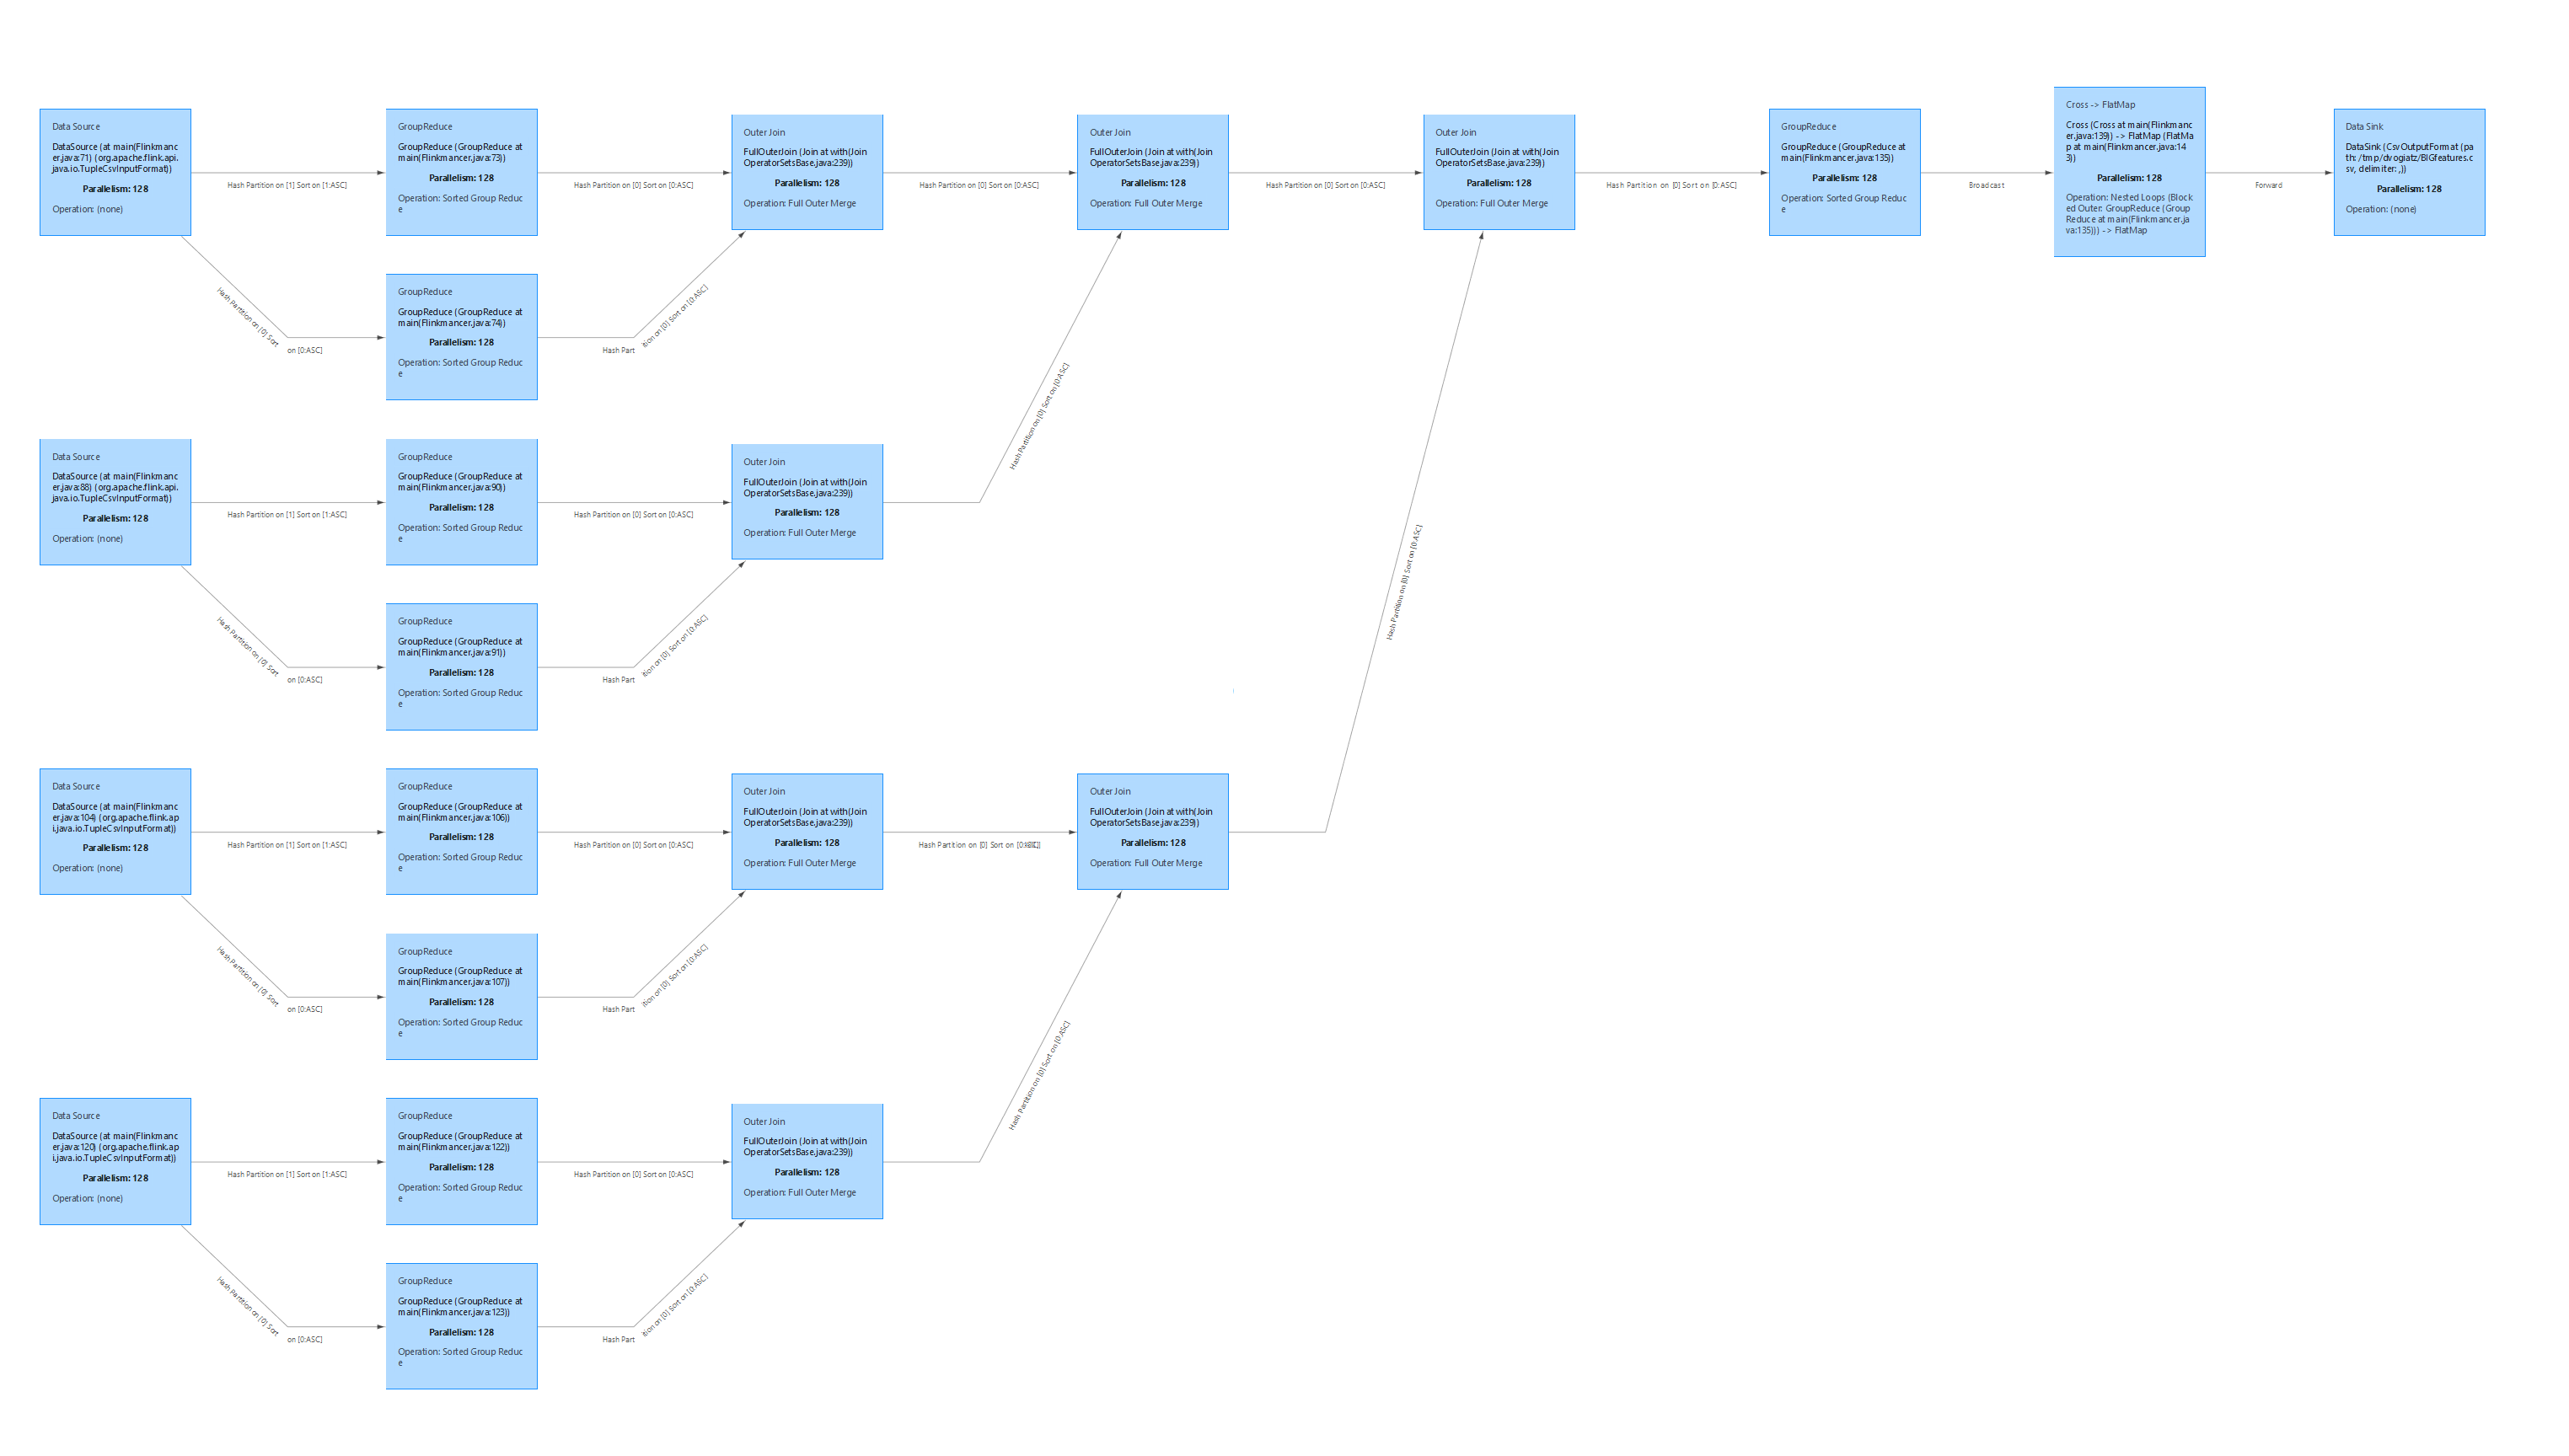
\includegraphics[width=\textwidth]{Thesis/images/diagram.png}}
\caption{Every process that takes place in the project}
\label{fig:graph}
\end{figure}

\chapter{Results}

\section{Experiment 1}
\begin{figure}[ht]
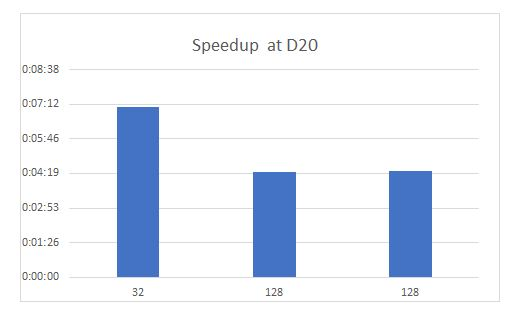
\includegraphics[width=10cm]{Thesis/figures/graph1.JPG}
\caption{Sppedup at D20 dataset from 32 to 128 cores}
\label{fig:graph}
\end{figure}



\section{Experiment 2}

% Replace with your text
%https://www.tablesgenerator.com/?fbclid=IwAR0W039IFX2-HUWOTwVTY_-CraF2DvdBtIlM6pCGMOZHgLBfQkyjM_V5TZY
%\chapter{Discussion}

\lipsum  % Replace with your text

\chapter{Conclusions and Future Work}

\section{Conclusions}
To sum up, in this thesis we created an Apache Flink application that can achieve both weak and strong scaling. We managed to extract features on large size input and showed that we can achieve it on even larger scale when the hard disk space issues are solved. We also showed that it is possible to speed up the process by increasing our resources.  We believe that this project will provide a useful tool for data analysis in the feature.
\section{Future Work}
The immediate work that shall be done is to use the features extracted here and train Logistic Regression models to help with Link Prediction.


% -------------------------------------------------------------------
% Bibliography
% -------------------------------------------------------------------

\bibliographystyle{plainnat}
\bibliography{main} 
[1] K. Sotiropoulos, J. W. Byers, P. Pratikakis, and C. E. Tsourakakis. Twittermancer: Predictinginteractions on twitter accurately.arXiv preprint arXiv:1904.11119, 2019.\newline
[2] DiGangi EA, Moore MK, editors. 2012. Research methods inhuman skeletal biology. Oxford: Academic Press.\newline
[3] J. Leskovec, D. Huttenlocher, and J. Kleinberg, “Predicting positive and negative links in online social networks,” in Proceedings of the 19th International Conference on World Wide Web. ACM, 2010, pp. 641–650.
% -------------------------------------------------------------------
% Appendices
% -------------------------------------------------------------------

%\begin{appendices}
%\chapter{Run and Configurations}

In order to run the project, there are some requirements:
Download Apache Flink 1.10.1 for Scala 2.12

After the downloaded archive is unpacked, flink has to be configured for the standalone cluster. The ``/conf" directory has 2 important files.
\begin{itemize}
\item flink-conf.yaml:

In this file we set: 
\newline ``jobmanager.rpc.address"  to be the IP of Job Manager. 
\newline ``taskmanager.memory.flink.size" to be the highest available DRAM. 
\newline ``taskmanager.memory.off-heap.size" to at least 1024m. 
\newline ``taskmanager.numberOfTaskSlots" to the number of cores each machine has. 
\newline ``taskmanager.memory.network.min" and ``taskmanager.memory.network.max" 
\newline in a way that flink.size * network.fraction (0.1) is between min and max.

\item slaves:

In this file we add the id of each machine that will run a task manager. 
\end{itemize}
Now we can start our cluster and run the project
\begin{itemize}
\item  “./flink-1.10.0/bin/start-cluster.sh" 
\item  “./flink-1.10.0/bin/flink run flinkmancer.jar -{}-cores [number of total cores] -{}-path [path to dataset] -{}-outpath [path to output file inclunding the name]" 
\end{itemize}

The data sets needs to be in ./data/{layer} for each different layer used. \newline 
In our test runs we used 4 different layers, ``follow", ``reply", ``quote", ``retweet".
After the program is executed , it produces a Features.csv file, containing 100 Features about each Edge of Vectors (each Vector being a user) and their common neighbors. 

%\chapter{Another Appendix}

\lipsum[1-3]  % Replace with your text

%\end{appendices}

\end{document}
